
Parámetros del test: 
Cantidad de iteraciones por filtro-version 20.
ALFA 150

\begin{figure}[h]
  \begin{center}
	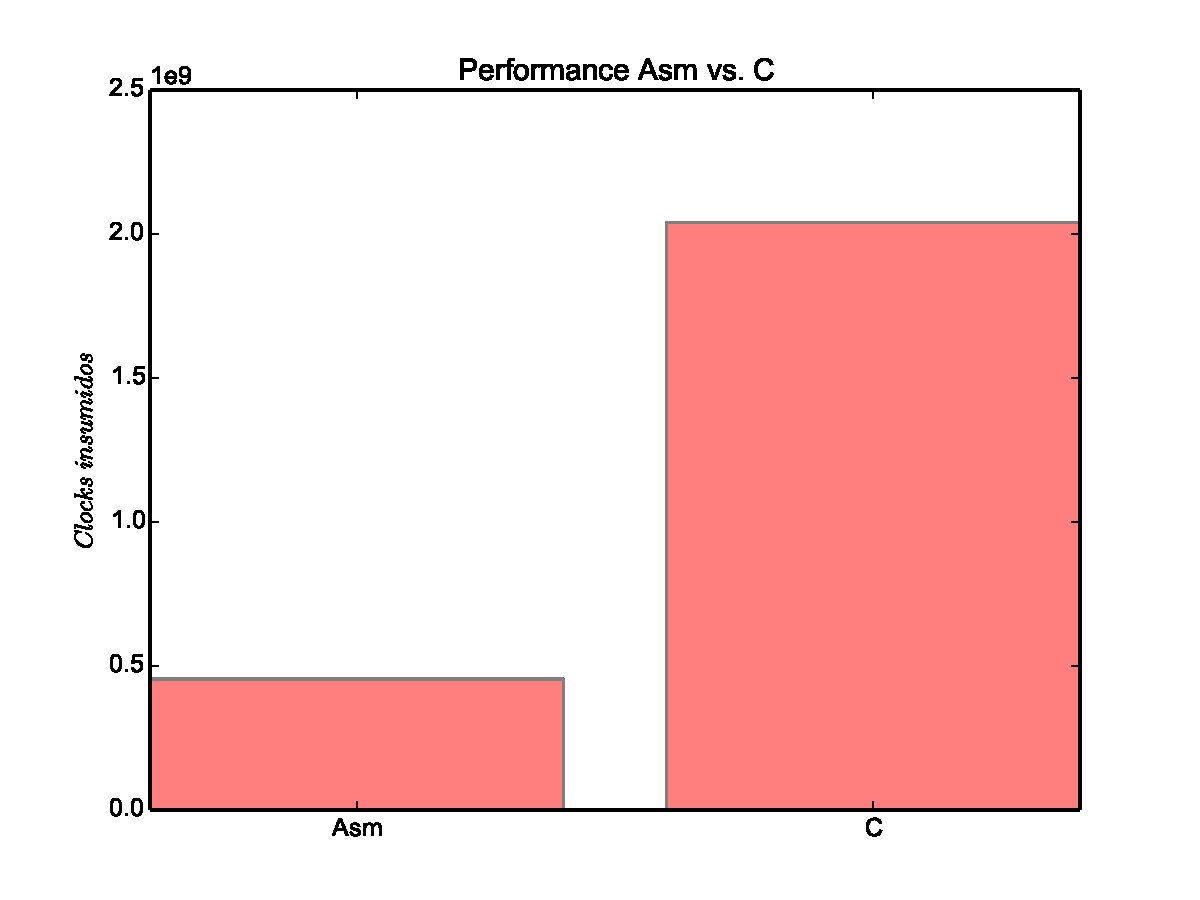
\includegraphics[scale=0.5]{ldrA.pdf}
	\caption{Test A}
  \end{center}
\end{figure}

$A)$ $assembler$ supera claramente a la version implementada en $C$. Claramente los accesos no suponen un problema, dado que por principo de vecinidad espacial, en la cache al leer un pixel, se traera consigo varios contiguos. La diferencia radica en el procesamiento paralelo que SIMD nos permite.

\begin{figure}[h]
  \begin{center}
	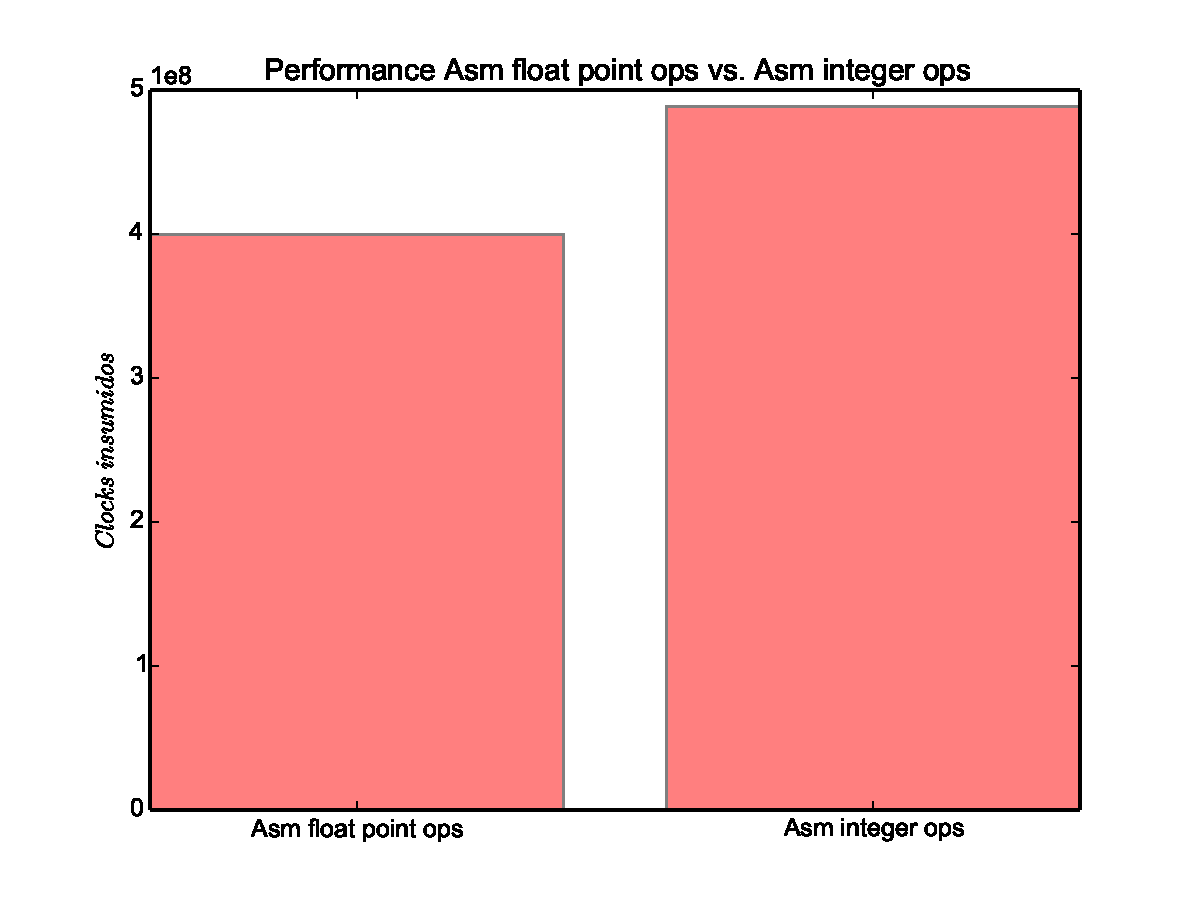
\includegraphics[scale=0.5]{ldrB.pdf}
	\caption{Test B}
  \end{center}
\end{figure}

$B)$ La version con operaciones en punto flotante insume menor cantidad de clocks del reloj que la version con operaciones en enteros: Para este caso particular, al menos, el hecho de tener que dividir cada escalar por separado no supone una ventaja, todo lo contrario. Y al final es más conveniente operar en punto flotante, dado que ya veniamos procesando en paralelo. Esto es particular a la implementación y a los cambios requeridos. Muy probablemente si se hubiese llevado a cabo en $sepia$ hubiese arrojado otros resultados, debido a que podriamos operar con enteros sin perder paralelismo.

